\chapter{Discussion}
This chapter discusses the challenges, processes and decisions through out the research. The main topics of this discussion is the limitation of wi-fi scope, how the events were triggered, why human analysis was selected and the reason to exclude the complexity of eavesdropping. 

\section{Collection of Wi-fi Traffic}
The selected TP-Link access point had Internet group management protocol (IGMP) \cite{igmp_rfc2236} default enabled. This protocol enables devices on a local network to subscribe to different multicast groups. Return traffic will then be addressed to the multicast group and not device's MAC address. Due to this functionality, only the outbound traffic generated form the robot vacuum cleaner was captured during the standby event. Initial analysis of the standby traffic verified this, when WLAN base filter was applied. These findings are presented in Figure \ref{fig:WLANIGMP_enabled}

\begin{figure}[H]
    \centering
    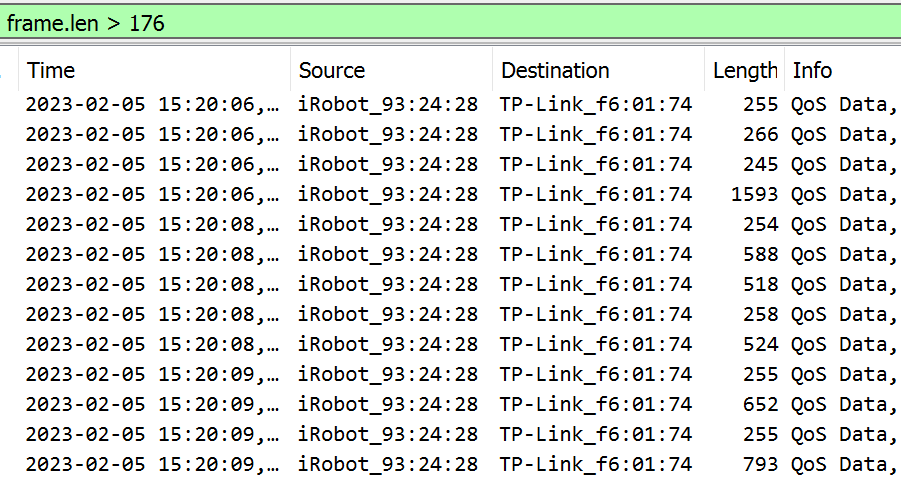
\includegraphics[width=0.8\textwidth]{figures/WLAN_IGMP_enabled.png}
    \caption{Wireshark WLAN capture, included basefilter and enabled IGMP}
    \label{fig:WLANIGMP_enabled}
\end{figure}

If IGMP enabled wi-fi would to be in the scope of this thesis, a process of filtering based on multicast group addresses should have been implemented. We therefore did a 20 minutes application triggered capturing in Oslo. Capturing only traffic including the MAC address to the access point. The capture included 9342 packets, which is 340\% more then LAN traffic average for the same event. By applying Wireshark filter, excluding all traffic except Irobot and multicast MAC addressed, we identified the new IGMP traffic flow. This is shown in Figure \ref{fig:WLANIGMP_all_enabled}. 

\begin{figure}[H]
    \centering
    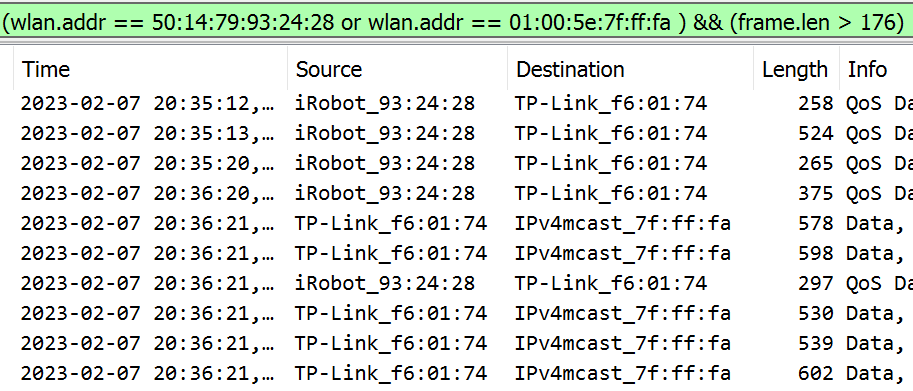
\includegraphics[width=\textwidth]{figures/WLAN_IGMP_ALL.png}
    \caption{WLAN IGMP application triggered cleaning test in Oslo}
    \label{fig:WLANIGMP_all_enabled}
\end{figure}

This increases the complexity of the filtering mechanisms. Identification of this multicast traffic would be simple in Oslo and Drammen, since only the Irobot roomba i7 is connected. The complexity occurs when more then one IoT device is connected to the same network. Devices can subscribe to the same or a new multicast group, making the wireless environment more complex and hard to navigate in. 

IGMP is not a standard protocol used in wi-fi networks \cite{wifi_ieee80211}, it would also increases the complexity of capturing, filtering and analysis in this thesis. We therefore decided to exclude IGMP wi-fi from this thesis and disabling the protocol on the access-point. 

\section{Event triggering}
As shown in Table \ref{tab:TestMatrixEnv1} and \ref{tab:TestMatrixEnv2}, several events was triggered in the same day and with limited standby window between them. The reason for this is the thesis' time constrains and the availability of smart environments. This increases the possibility of cross event influence, especially in the end of cleaning reporting from the Irobot vacuum cleaner. To mitigate the influence insecurity, we decided to only focus on the event initiation and not the end of cleaning reporting. Event triggering traffic is assumed to be the same regardless of previous events. 

Another disadvantage is that a real life simulation is not possible. There will not be triggered 5 cleaning events, within 2 hours. Event triggering timestamps will appear unrealistic, since we assume that users do not set a timer to trigger cleaning. Timestamps captured and identified in this research can therefore not be used in attributing events, but could increase the confident if captured in a real smart environment. 

We therefore decided that only the event triggering and reoccurring signatures will be included in this research. The amount of traffic sent after cleaning could be influenced by the unrealistic triggering pattern of this research. 

\section{Method of Analysis}
Both human based analysis and ML were discussed as the traffic analysis method for this thesis. As mentioned in related work, several other researches have used ML to extract information from network traffic. During the literature review, we did not find any documentation on who the robot vacuum cleaner communicated, which protocols were used, and if anything was visible in the capture files. Ether way the data would have to be pre-processed by a human to identify which attributes that could be used in further analysis.

This thesis aimed to identify the level of knowledge an attacker would need to have to be able to expose private information. We believe that with the use of human based analysis, this is better identified. Due to the level of abstraction that ML would introduce. 

The authors background is more in the desertion of telecommunication rather then data science. ML would therefore introduce another abstraction, which would decrees the ability to implement and evaluate analysis of data. Based on these factors as well as the thesis' time constrains, we decided to use human based learning to do the analysis. 


\section{The Complexity of Eavesdropping}
The level of complexity to conduct and eavesdropping attack for WLAN, LAN or WAN is not addressed in this thesis. This is a topic which should be addressed in separate research, due to the variety of devices and configurations, in different smart environments. We decided to create a simple smart home environment, to best address the research questions with the least amount of network infrastructure complexity. 

In wireless eavesdropping an attacker would only need to be in wireless range of the access point and the IoT device to collect corresponding network traffic. Eavesdropping devices can be placed in the vicinity of the smart environment, or installed inside the environment. Data could be stored locally or exported to a online service through Internet connection. 

For LAN and WAN eavesdropping the attacker would need physical access to the local network, or exploit remote access to network devices. These operations challenges both physical and technical security and is therefore out of scope for this thesis. 

